\section{Planteamiento del Problema}

En el contexto de la Web Semántica, y con el soporte de las Arquitecturas Orientadas a
Servicios (SOA), el número de fuentes de datos y servicios Web ha explotado en
los últimos años. Por ejemplo, la colección de bases de datos de biología
molecular actualmente contiene 1.170 bases de datos~\cite{Galperin09}, un número
que es
mayor que el del último año por 95~\cite{Galperin2008}, y que el de hace dos
años por 110~\cite{Galperin2007};
las herramientas y servicios, así como el número de instancias
publicados por estos recursos, siguen una progresión similar~\cite{Benson07}.
Gracias a
esta variedad de datos, la tendencia de los usuarios es hacia depender cada vez
más de métodos automáticos para manejarlos tales como recuperación de datos de
fuentes públicas y análisis utilizando herramientas o servicios Web compuestos
en flujos de trabajo complejos.

La SOA típica consiste de dos capas. La capa concreta que está hecha de
servicios concretos cuyas funcionalidades son descritas en términos de pre- y
post-condiciones y propiedades no funcionales en conjuntos de parámetros de
calidad de servicio (QoS), y
la capa abstracta compuesta de aplicaciones de software cuyas funcionalidades
son descritas en términos de flujos de trabajo abstractos y propiedades no
funcionales en términos de restricciones de QoS. La ejecución de un flujo de
trabajo abstracto involucra la instanciación de los servicios abstractos en
servicios concretos que cumplan con los requerimientos funcionales y no
funcionales. Este proceso de instanciación puede ser visto como una búsqueda de
una instanciación objetivo en el espacio combinatorio de todas las
instanciaciones válidas. Entonces se está interesado en técnicas eficientes para
realizar esta búsqueda que sean capaces de escalar a medida que el número de
servicios concretos o la complejidad del flujo de trabajo aumenta. Se llama al
problema de instanciar un flujo de trabajo dado con servicios concretos de un
conjunto de servicios concretos dado, de manera que ciertas demandas de QoS sean
cumplidas, el Problema de Instanciación de Flujos de Trabajo (WIP).

En este trabajo se considera una versión restringida de WIP que adopta el
enfoque Local-As-View (LAV) \cite{levy:bucket}. En LAV, todos los elementos de un
problema son especificados con un lenguaje común basado en servicios abstractos
tal que los servicios concretos se describen como vistas de servicios
abstractos, la calidad de una instanciación como una función de utilidad global
que combina los diferentes parámetros QoS, y el flujo de trabajo abstracto como
una consulta conjuntiva sobre los servicios abstractos; esta representación es
similar a la que es generada de manera semiautomática para el sistema DEIMOS
\cite{AmbiteISWC09}. En esta versión de WIP, las reglas que definen flujos de trabajo
(consultas conjuntivas) y servicios concretos (vistas) son creados de manera que
todas las restricciones funcionales sobre pre- y post-condiciones de los
servicios y sus combinaciones sean satisfechas, y las medidas de QoS son
representadas anotando cada descripción de servicio concreto con un número real
que representa la utilidad QoS global del servicio.

Bajo estas suposiciones, WIP puede ser convertido en el bien conocido Problema
de Reescritura de Consultas (QRP) para LAV que es central a los sistemas de
integración \cite{halevy:survey}. QRP consiste de una consulta conjuntiva que debe ser
respondida en términos de vistas donde la consulta y las vistas son descritas
usando LAV con relaciones abstractas. Este problema es importante en el contexto
de integración de datos \cite{Chen05,JaudoinPRST05}, y optimización de consultas y mantenimiento
de datos \cite{AfratiLU07,levy:bucket}, y varias soluciones que escalan a un número grande de
vistas han sido definidas \cite{arvelo:aaai06,pods:DuschkaG97,sac:DuschkaG97,levy:bucket,pottinger:minicon}.

La solución propuesta por Arvelo et al. \cite{arvelo:aaai06} está basada en la enumeración
eficiente de modelos de una teoría lógica proposicional. Dada una consulta conjuntiva, una teoría
lógica es construída de manera que cada modelo de la teoría codifica una
reescritura válida, y así todas las reescrituras son obtenidas enumerando los
modelos de la teoría. Esta enumeración puede ser realizada eficientemente si la
teoría lógica está en cierta forma normal llamada la forma normal de negación
determinística y descomponible (d-DNNF) \cite{darwiche:d-dnnfs}. Así,
la solución consiste en transformar (llamado compilar en el campo de
compilación del conocimiento) la teoría lógica en el formato d-DNNF para
enumerar sus modelos eficientemente.

Pero las teorías d-DNNF no sólo soportan la enumeración eficiente de sus
modelos, sino también otras operaciones. Entre ellas se encuentra la enumeración
de los modelos con mejor calidad. Dada una función de calidad de literales
$r(\ell)$ que asigne calidades a cada literal $\ell$, se define la calidad
$r(\omega)$ de un modelo $\omega$ como la suma de las calidades de los literales
activados por $\omega$ (es decir,
$r(\omega)\doteq\sum_{\omega\vDash\ell}r(\ell)$), y se dice que $\omega$ es un modelo
de mejor calidad si no hay modelo $\omega'$ tal que $r(\omega')<r(\omega)$.

Dada una teoría en d-DNNF, se computa la calidad de los mejores modelos, y
los mejores modelos, en tiempo lineal en el tamaño del d-DNNF. Este cómputo
transforma el GAD del d-DNNF en un circuito aritmético reemplazando los nodos
AND con `+' y los nodos OR con `min'. La función de calidad de literales
asigna valores a las hojas del circuito aritmético (grafo acíclico dirigido usado
para calcular polinomios) que son propagados a la raíz en tiempo
lineal. El valor de la raíz es la calidad del mejor modelo \cite{darwiche:weighted}.

En este trabajo se propone explotar las propiedades de los d-DNNF construyendo una
teoría lógica cuyos modelos codifican las instanciaciones del flujo de trabajo
y cuyos mejores modelos codifican las instanciaciones óptimas (mejores). Así, la
búsqueda combinatoria se reduce a la computación de un mejor modelo de una
teoría lógica que puede ser realizada eficientemente una vez que la teoría es
transformada al formato d-DNNF.

\subsection{Trabajo Relacionado}

En esta sección se resumen los enfoques existentes que proveen soluciones
a los problemas de selección de servicios y reescritura de consultas y se
discute el trabajo relacionado en el área de inteligencia artificial llamado
compilación del conocimiento.

\subsubsection{Selección de Servicios}

El problema de seleccionar los servicios que implementan un flujo de trabajo
abstracto y cumplen mejor los criterios basados en QoS es conocido como el
problema de selección o composición de servicios consciente de QoS, que ha sido
demostrado ser \emph{NP-hard} \cite{Hiroshi2008}. Este es un problema de optimización
combinatoria y varias heurísticas han sido propuestas para conseguir una
solución relativamente buena en un período razonable de tiempo.

Rahmani et al. \cite{rahmani08} presentan una heurística basada en una métrica de distancia
que guía un algoritmo de búsqueda; esta métrica induce un orden de
los servicios en una manera en que los nodos vertedero (sin salida) tienen baja probabilidad
de ser visitados. En una serie de artículos, Berardi y otros \cite{berardi05,berardi08,berardi06}
describen
servicios y flujos de trabajo en términos de máquinas de estados finitos
determinísticas que son codificadas usando teorías de Lógicas Descriptivas
cuyos modelos corresponden a soluciones del problema. Aunque se podrían explotar
métodos para formalismos de Lógicas Descriptivas, no han sido reportados la
escalabilidad o el rendimiento de la solución propuesta.

Ko et al. \cite{myoung08} proponen un enfoque basado en restriccciones que codifica
los valores permisibles no funcionales como un conjunto de restricciones cuya
violación debe ser minimizada; para recorrer el espacio de soluciones
posiblemente óptima, se implementa un algoritmo híbrido que combina las
metaheurísticas \emph{tabu search} y \emph{simulated annealing}. Los resultados
experimentales muestran que la solución propuesta es capaz de escalar a un
número grande de servicios y procesos abstractos. Cardellini et al. \cite{cardellini07}
codifican una parte del problema de composición de servicios caracterizados por QoS
como un problema de programación lineal \cite{cardellini07}. Por otra parte, Wada et al.
\cite{Hiroshi2008} trata el problema como uno de optimización con múltiples objetivos donde
los diferentes parámetros de QoS son considerados igualmente importantes en vez
de ser agregados en una función. Luego se propone un algoritmo basado en
algoritmos genéticos que identifica un conjunto de composiciones de servicios
no dominadas que mejor satisfacen los requerimientos QoS.

Alrifai y Risse \cite{alrifaiR09} proponen una solución de doble cara que usa un
algoritmo de programación entera híbrido para obtener la descomposición de QoS
globales en restricciones locales y luego selecciona los servicios que mejor
cumplen las restricciones locales.

Recientemente, dos soluciones basadas en planificación han sido propuestas.
Kuter y Golbeck \cite{kuterG09} extienden el algoritmo de planificación SHOP2 para
seleccionar la composición confiable de servicios que implementan un modelo de
procesos OWL-S dado, mientras que Sohrabi y McIlraith \cite{sohrabiM09} proponen una
solución basada en planificación HTN donde las métricas de preferencia del
usario y regulaciones de dominio son utilizadas para guíar el planificador hacia
el espacio de composiciones relevantes. Finalmente, Lécué \cite{lecue09} propone un
algoritmo basado en genética para identificar la composición de servicios que
mejor cumple con los criterios de calidad para un conjunto de parámetros QoS.

Aunque estas soluciones son capaces de resolver el problema de optimización y
escalar a un número de procesos abstractos, ninguno de ellos está ajustado para
describir semánticamente los servicios en términos de procesos abstractos, ni
para usar estas descripciones para identificar los servicios que implementan un
flujo de trabajo dado o que mejor cumplen los criterios no funcionales del
usuario.

\subsubsection{Reescritura de Consultas}

Un número de algoritmos han sido desarrollados para encontrar las reescrituras
de una consulta dada; los más prominentes son el algoritmo \emph{bucket} \cite{levy:bucket}, el
algoritmo de reglas inversas \cite{pods:DuschkaG97,Qian96}, el algoritmo
\minicon \cite{pottinger:minicon}, y el
algoritmo \mcdsat \cite{arvelo:aaai06}. Generalmente, la reescritura de consultas trabaja en
dos fases. Durante la primera, el algoritmo identifica las vistas que reescriben
al menos un subobjetivo de la consulta, y durante el segundo estas reescrituras
parciales son combinadas en reescrituras completas. La diferencia principal
entre los algoritmos es el conjunto de criterios usado para elegir las vistas
relevantes para reducir el espacio de reescrituras no útiles.

El algoritmo denominado \emph{bucket} reduce el número de posibilidades considerando sólo cada
subobjetivo de la consulta aislado, y seleccionando las vistas que son capaces
de producir al menos los atributos proyectados por la consulta. Como los
atributos involucrados en los \emph{joins} de la consulta no son verificados, un número
grande de reescrituras comprendido por productos cartesianos puede ser generado.

El algoritmo de reglas inversas construye un conjunto de reglas que invierten
las definiciones de vistas y establecen cómo computar tuplas para las relaciones
de la base de datos a partir de las tuplas de las vistas. Al igual que el algoritmo
bucket, puede producir un gran número de reescrituras no útiles.

El algoritmo \minicon\ supera las limitaciones de los algoritmos previos
identificando solamente vistas que reescriben un conjunto de los subobjetivos de
la consulta, y que pueden ser combinados con el resto de los subobjetivos. La
idea principal es identificar las asociaciones entre variables de cada
subobjetivo a las variables en uno o más subojbetivos en las vistas, de manera
que las variables de \emph{join} de la consulta son asociadas a las variables de
\emph{join}
del cuerpo de una vista o a variables distinguidas de la vista. Asociaciones
entre variables y subojbetivos son representadas en las llamadas \emph{MiniCon
Descriptions} (MCDs) \cite{pottinger:minicon}.

Finalmente, el algoritmo \mcdsat\ es capaz de identificar las reescrituras de una
consulta traduciendo el problema de reescritura al problema de enumeración de
modelos de una teoría proposicional cuyos modelos están en correspondencia con
las reescrituras de la consulta. El algoritmo explota las propiedades de los
d-DNNF para enumerar eficientemente los modelos de la teoría.
El algoritmo
\mcdsat\ ha demostrado escalar mejor que el algoritmo \minicon\ sobre un número
grande de experimentos donde frecuentemente muestra mejoras de rendimiento de
varios órdenes de magnitud. Sin embargo, el algoritmo \mcdsat\ no fue diseñado
para problemas de reescritura que involucren constantes explícitas, ni para
computar las mejores reescrituras respecto a una función de utilidad o modelo de
costo dado. En este trabajo se propone una codificación extendida que supera
estas limitaciones y se aplica la codificación al problema de instanciación de
flujos de trabajo.

\subsubsection{Compilación del Conocimiento}

Compilación del conocimiento es el área en inteligencia artificial que se ocupa
del problema de traducir teorías lógicas en fragmentos apropiados que hagan
tratables ciertas operaciones deseadas \cite{cadoli:compilation}. Diferentes lenguajes de
compilación han sido definidos. Por ejemplo están los \emph{Ordered
Binary Decision Diagrams} (OBDDs) \cite{bryant:obdd},
\emph{Negation Normal Form} (NNF) \cite{barwise:handbook}, y
\emph{Decomposable Negation Normal Form} (DNNF) \cite{darwiche:map}. En este trabajo se usan las
propiedades de los DNNF determinísticos (d-DNNF) \cite{darwiche:d-dnnfs} para proveer una
solución eficiente y escalable al problema de selección de servicios.

\begin{figure}[t]
\centering
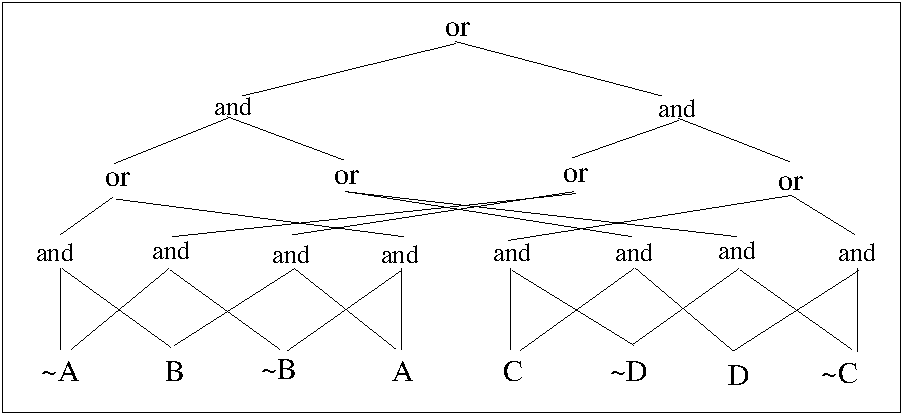
\includegraphics[width=.7\textwidth]{graphics/odd}
\caption{Un NNF descomponible y determinístico.}
\label{fig:dnnf}
\end{figure}

Una teoría en Negation Normal Form es construida desde literales usando sólo
conjunciones y disjunciones \cite{barwise:handbook}, y puede ser representada como un grafo
acíclico dirigido en que las hojas son etiquetadas con literales y los nodos
internos con $\land$ y $\lor$; ver ejemplo en la figura~\ref{fig:dnnf}. Esta
forma normal es universal, lo que significa que para cada fórmula lógica hay una
equivalente en formato NNF. Se dice que un NNF es descomponible (DNNF)
\cite{darwiche:d-dnnfs}
si para cada conjunción $\bigwedge_i\phi_i$, sus variables son disjuntas por pares; es
decir, $Vars(\phi_i)\cap Vars(\phi_j)=\empty$ para $i\neq j$. Un DNNF soporta un
número de operaciones en tiempo polinomial en el tamaño de su GAD. Por ejemplo,
podemos probar si un DNNF es satisfactible haciendo un sólo recorrido 
sobre su GAD en tiempo linear. Se dice que un DNNF es
determinístico (d-DNNF) \cite{darwiche:d-dnnfs} si para cada disjunción $\bigvee_i\phi_i$, los
disjuntos son lógicamente contradictorios por pares, es decir,
$\phi_i\land\phi_j\equiv\textbf{false}$ para $i\neq j$.
El NNF en la figura~\ref{fig:dnnf}, por ejemplo, es
descomponible y determinístico. Un d-DNNF soporta conteo de modelos en
tiempo polinomial en el tamaño de su GAD, y enumeración de modelos en tiempo
polinomial en el tamaño de la salida. Además, dada una función de calidad de
literales $r$, se puede computar la calidad del mejor modelo en tiempo
polinomial para DNNFs \cite{darwiche:weighted}.

Toda teoría puede representarse en las formas DNNF y d-DNNF pero traducir una teoría CNF a
formato DNNF tiene costo exponencial en el peor caso. Esta traducción se
llama compilación en este campo. Hay un compilador públicamente disponible,
llamado c2d\footnote{\url{http://reasoning.cs.ucla.edu/c2d}}, que realiza este proceso de compilación y que hace uso
de técnicas de SAT modernas como backtracking dirigido por conflictos,
aprendizaje de cláusulas y caching \cite{darwiche:compiler}. Este compilador incurre en el peor
caso (peor gasto) en espacio exponencial en un parámetro llamado el ancho del árbol de
descomposición que está relacionado a la ``conectividad'' de la teoría CNF.
Sin embargo, en nuestros experimentos, las teorías CNF que son compiladas son de
ancho pequeño.

\subsection{Formalización}

Consideramos catálogos de servicio de la forma $C=\tup{S,T}$ donde $S$ es un
conjunto de predicados que representa servicios abstractos y $T=\{T_s\}_{s\in S}$ es una
colección de tablas que representa el resultado de evaluar los servicios
abstractos. En el contexto del WIP, un catálogo de servicio $C$ es una
descripción virtual de la salida producida por flujos abstractos
implementados por servicios concretos descritos como vistas. Un flujo de trabajo
$W$ sobre $S$ es una consulta conjuntiva de la forma

\[ W(\vvec{x})\ \qrule\ s_1(\vvec{x}_1),\,s_1(\vvec{x}_2),\,\ldots,\,s_m(\vvec{x}_m)\,, \]

donde $s_i\in S$, $\vvec{x}$ es un vector de variables y cada $\vvec{x}_i$ es un vector de variables y
constantes. El resultado de $W$ sobre $C$, denotado como $W(C)$, es la tabla con
 $|\vvec{x}|$ columnas que resulta de la proyección del \emph{join} relacional
$\join\!\!\{T_{s_i}\}_{i=1}^n$ sobre $\vvec{x}$. Los átomos en el cuerpo de $W$ son llamados los
(sub)objetivos de $W$, y las variables en la cabeza de $W$ son llamadas
distinguidas.

Un servicio concreto es descrito como una vista $V$ sobre $C$ que, siguiendo
LAV, es una consulta sobre $S$. Dado un catálogo $C$, un flujo de trabajo $W$ y
una colección de $n$ vistas $E=\tup{\{V_i\}_{i=1}^n,\{E_i\}_{i=1}^n}$, se pide
conseguir todas las tuplas en
$W(C)$ que puedan ser obtenidas de vistas en $E$. Es decir, se necesitan
conseguir las \emph{instanciaciones}

\[ R(\vvec{x})\ \qrule\ V_{i_1}(\vvec{x}_1),\,V_{i_2}(\vvec{x}_2),\,\ldots,\,V_{i_{m_i}}(\vvec{x}_{m_i}) \]

tales que $R(E) \subseteq Q(C)$.
Un problema de instanciación de flujo de trabajo es una
tupla $\tup{S,W,\{V_i\}_i}$ donde $S$ es un conjunto de predicados
que representa servicios
abstractos, $W$ es un flujo de trabajo sobre $S$, y $\{V_i\}_i$ una colección de vistas
que define servicios concretos. Suponemos trabajo con problemas \emph{seguros}
en el sentido en que todas las variables mencionadas en la cabeza del flujo de
trabajo (respectivamente en la cabeza de cada vista) aparecen en el cuerpo del
flujo de trabajo (respectivamente en el cuerpo de cada vista). Además, sólo
lidiamos con WIPs sin predicados aritméticos dentro del flujo de trabajo o
vistas. Una instanciación $R$ es \emph{válida} si para todos los catálogos $C=\tup{S,T}$ y
extensiones $\{E_i\}_i$, $R(E)\subseteq Q(C)$. Una colección $\R$ de instanciaciones válidas es una
solución si para todos los catálogos de servicio $C=\tup{S,T}$ y extensiones $\{E_i\}_i$, no
existe $\R'$ tal que $\R(E)\subset\R'(E)\subseteq Q(C)$.

\subsubsection{Teorías Lógicas}

Se usa una solución similar a la descrita en
\cite{arvelo:aaai06} para codificar el WIP. 
Se identifican instanciaciones del flujo de trabajo enumerando los modelos de
una teoría lógica
$\Delta=\Delta_{com}\cup\Delta_{id}^1\cup\cdots\Delta_{id}^N$
donde $\Delta_{com}$ especifica cómo combinar $N$ copias independientes de la teoría
$\Delta_{id}$ que cubren los objetivos en $W$.
Cada $\Delta^i_{id}$ es una copia etiquetada $\Delta_{id}$ en la cual cada
literal 
$\ell$ está etiquetado como $\ell^i$.
La teoría \emph{Instantiation Description} (ID) $\Delta_{id}$ consiste de
diferentes grupos de cláusulas que garantizan que sus modelos están en
correspondencia con instanciaciones parciales, mientras que la teoría
$\Delta_{com}$ contiene cláusulas adicionales para garantizar una combinación
correcta y completa de instanciaciones parciales para una instanciación
completa.
La teoría ID $\Delta_{id}$ consiste de las siguientes variables:

\begin{enumerate}[--]
\item $\{v_0,\ldots,v_n\}$ para indicar qué $V_i$ se usa, o $v_0$ para indicar el ID nulo.
\item $\{g_1,\ldots,g_m\}$ para indicar objetivos cubiertos por la vista.
\item $\{z_{j,k,i}\}$ para indicar que el objetivo $j$ en $W$ está cubierto por el objetivo $k$ en $V_i$.
\item $\{t_{x,y}\}$ para indicar que la variable/constante $x$ en $W$ está asociada a la variable/constante $y$ en la vista.
\end{enumerate}

Los rangos de los índices para las variables $z$ y $t$ dependen del problema.

Las siguientes cláusulas codifican el problema WIP en términos de los WIDs.
Rajaraman et al.\ \cite{RajaramanSU95} mostraron que para consultas sin negación
o comparaciones aritméticas, pero con constantes, y $m$ objetivos y $k$
variables en la cabeza del flujo de trabajo, es suficiente considerar
instanciaciones de longitud a lo más $N=m+k$.

\begin{enumerate}[C10.]
\item[C1.] (Al menos una vista es usada): $\bigvee_{i=0}^n v_i$.
\item[C2.] (A lo más una vista es usada): $\neg v_i\lor\neg v_j$ para $i\neq j$.
\item[C3.] (Vista nula implica nulidad): $v_0 \Rightarrow \neg g_j$ para $1\leq j\leq m$.
\item[C4.] (Las vistas son útiles): $v_i \Rightarrow \bigvee_{j=1}^m g_j$ para $1\leq i\leq n$.
\item[C5.] (Objetivos cubiertos máximo una vez): $z_{j,k,i} \Rightarrow \neg z_{j,l,i}$ para $i,j,k,l$ apropiados.
\item[C6.] (Alcance de las vistas): $v_i \Rightarrow \neg g_j$ para objetivos que no pueden ser cubiertos por $V_i$.
\item[C7.] (Consistencia): $v_i \land g_j \Leftrightarrow \bigvee z_{j,k,i}$ para $i,j,k$ apropiados.
\item[C8.] (Variables muertas): $v_i \Rightarrow \neg t_{x,y}$ para todo $x,y$ con $y\notin V_i$.
\item[C9.] (1-1 para $\exists$ vars): $v_i \land t_{x,y} \Rightarrow \neg t_{x,y'}$ para todas las variables existenciales $y,y'\in V_i$.
\item[C10.] (Distinguidos): $v_i \Rightarrow \neg t_{x,y}$ para $x$ distinguido y $y\in V_i$ existencial .
\item[C11.] (Existencial): $v_i\land t_{x,y}\Rightarrow g_j$ para exist.\ $y\in V_i$ y objetivos $g_j$ que contengan $x$.
\item[C12.] (Coincidencia): $v_i\land z_{j,k,i} \Rightarrow t_{x,y}$ para todo
$x,y$ que deban coincidir si $g_j$ es cubierto por el objetivo $k$ en $V_i$.
\item[C13.] (Si todas las variables en $V_i$ son distinguidas, sólo cubre un objetivo): $v_i \land g_j \Rightarrow \neg g_k$ para vistas $v_i$ apropiadas.
\end{enumerate}

Estas son las mismas cláusulas usadas por \mcdsat\ para codificar QRPs \cite{arvelo:aaai06}.
Para poder manejar símbolos constantes apropiadamente, las cláusulas deben ser
mejoradas con:

\begin{enumerate}[C10.]
\item[C14.] (Inconsistencia directa 1): $t_{x,A} \Rightarrow \neg t_{x,B}$.
\item[C15.] (Inconsistencia directa 2): $t_{A,x} \Rightarrow \neg t_{B,x}$.
\item[C16.] (Inconsistencia directa 3): $\neg t_{A,B}$.
\item[C17.] (Transitividad 1): $v_i\land t_{A,y}\land t_{x,y}\land t_{x,z}\Rightarrow t_{A,z}$.
\item[C18.] (Transitividad 2): $v_i\land t_{y,A}\land t_{y,x}\land t_{z,x}\Rightarrow t_{z,A}$.
\end{enumerate}

El problema principal al manejar constantes es estar seguro de que no haya dos
constantes distintas asociadas entre sí directa o indirectamente. Las cláusulas
C14--C16 quitan asociaciones directamente inconsistentes, mientras que las
últimas dos cláusulas implementan propagación de asociaciones restringida que
quita inconsistencias indirectas.
De la misma manera, la teoría $\Delta_{com}$ que especifica instanciaciones
completas contiene las siguientes cláusulas:

\begin{enumerate}[C10.]
\item[C19.] (Cubrir todos los objetivos): $\bigvee_{j=1}^m g^i_j$ para $1\leq i\leq N$.
\item[C20.] (Cobertura disjuntiva): $g^i_k \Rightarrow \neg g^j_k$ para $i\neq j$.
\item[C21.] (Quitar simetrías): $g^i_j \Rightarrow \bigvee_{k=1}^{j-1} g^{i-1}_k$
            para $1\leq j\leq m$ y $1\leq i\leq N$.
\item[C22.] (Inconsistencia directa 4): $t^i_{x,A} \Rightarrow \neg t^j_{x,B}$.
\end{enumerate}

Estas cláusulas proveen una caracterización correcta y completa de WIPs en el
sentido en que sus modelos están en correspondencia con las instanciaciones del
flujo de trabajo.

\subsubsection{Parámetros QoS}

Para los parámetros QoS, se supone un modelo de agregación aditiva simple en el
que cada vista
$V_i$ está asociada con un costo $c(V_i)$ (negativo si tratamos de utilidad),
y una instanciación completa con la suma de los costos de sus vistas.
Una instanciación óptima o mejor es una con costo mínimo, y el valor óptimo del
WIP es el costo de una instanciación óptima.
Un WIP siempre tiene un valor óptimo bien definido (si no hay instanciaciones,
su costo es $\infty$), pero puede tener múltiples mejores instanciaciones.
El WIP con costos consiste en encontrar todas las instanciaciones óptimas o una
instanciación, esto depende de la aplicación particular.
En la formulación propuesta, esto puede hacerse a partir del d-DNNF que codifica
$\Delta$
usando la función de calidad de literales $r$ que asigna
$r(\ell)=c(V_i)$ si
$\ell=v_i$, y $r(\ell)=0$ if $\ell\notin\{v_1,\ldots,v_n\}$.
